\documentclass[../main.tex]{subfiles}
\graphicspath{{\subfix{../images/}}}
\begin{document}
\section{The Pokémon Entreprise}

Parlons de la fameuse entreprise qui fabrique des \glspl{pokemon}, et dans laquelle j'ai fait mon stage.

\subsection{L'entreprise}
C'est une entreprise qui se trouve à Douai, qui existe depuis 2002, et qui vend et fabrique des \Glspl{pokemon}.

Elle s'appelle \textit{The Pokémon Company}.

\subsubsection{Les chiffres clés}
Elle a déjà vendu 2 millions de \Glspl{pokemon}. Elle compte 10 000 employés, tous fans de \Glspl{pokemon}.
Un organigramme est visible dans les annexes \figref{\ref{fig:organigramme}}.

\subsubsection{Sa spécialisation}
Thé Pokémon Entreprise ne vend pas n'importe quels \gls{pokemon}. Elle est spécialisée dans la quatrième génération.

\subsubsection{Ses produits dérivés}
Elle vend aussi des \glspl{pokeball}\footnote{Le terme "Pokéball" vient de la contraction entre "Pokémon" et "Ball".}, des biscuits pour pokémon, ou encore des \acrfull{ct}, ce qui lui permet de diversifier ses ventes.

\subsection{Positionnement sur le marché}

La quatrième génération est sortie le 28 septembre 2006, et compte 107 nouveaux pokémon, ainsi que 113 nouvelles attaques\citer{4g}.

The Pokémon Entreprise a quelques concurrents, notamment Gum Freak, mais a The Pokémon Entreprise a su percer le marché grâce à sa grande variété de Pokémon de type eau, dont Tiplouf, qui mesure tout de même 40cm de haut\citer{tiplouf}.

\subsection{Son avenir}

L'entreprise compte construire un autre bâtiment pour s'agrandir. Un aperçu est disponible dans les annexes \figref{\ref{fig:batiment}}.

Elle compte aussi diversifier les différents pokemon électrique, qui est un marché porteur en ce moment.
Image du futur pokémon électrique qui sait aussi versionner ses projets informatiques : \textit{Gitar} \figref{\ref{fig:gitar}}.


\begin{figure}[h]
    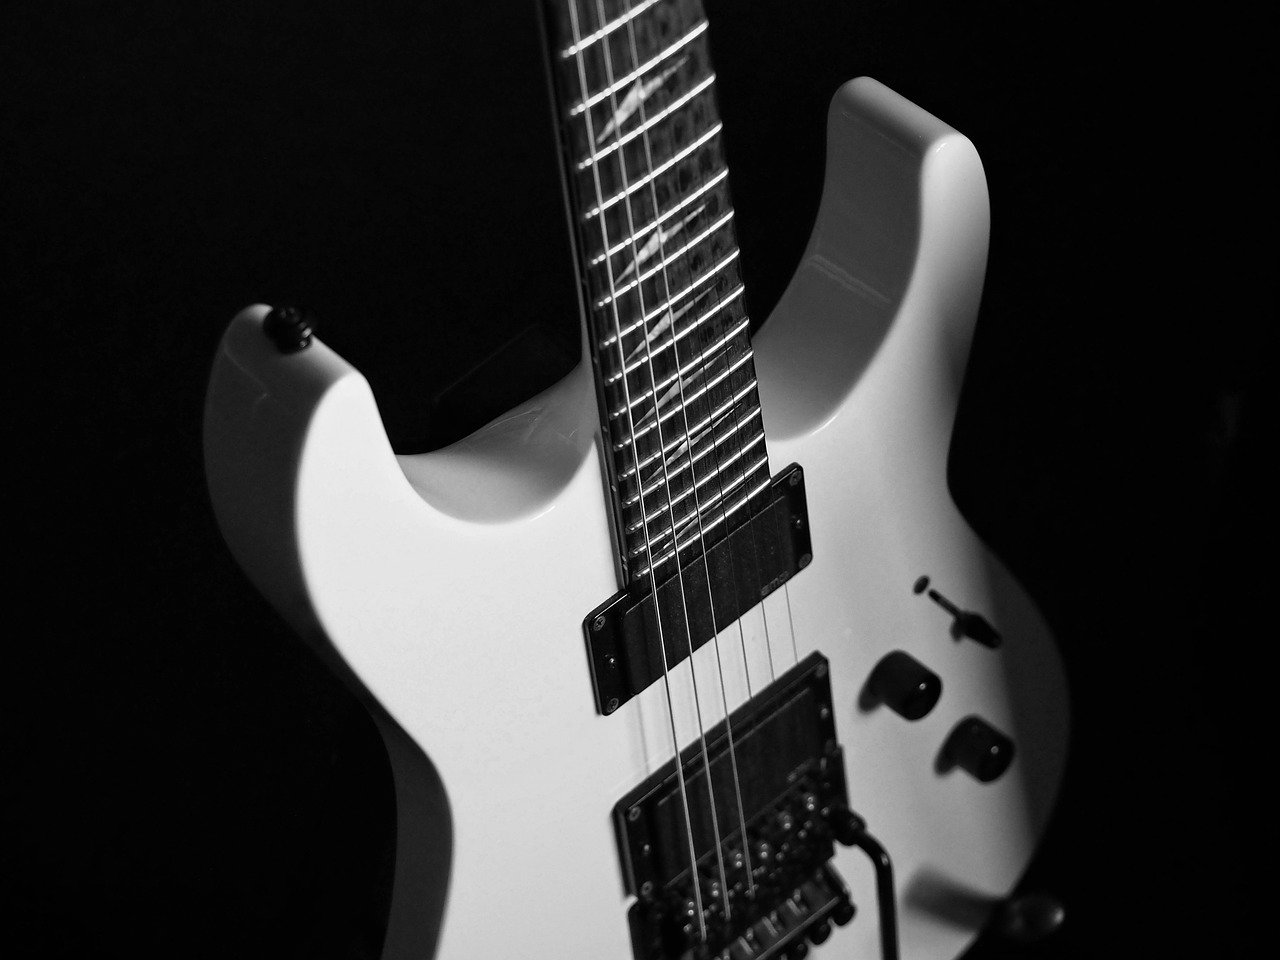
\includegraphics[width=0.3\linewidth, center]{images/pokemons/gitar}
    \captionsetup{font=small,labelfont=bf, justification=centering}
    \caption{Aperçu du futur pokémon électrique "Gitar"}
    \label{fig:gitar}
\end{figure}

\end{document}